% !TEX root = main.tex
\section{Design Description}
\label{sec:design_description}
Figure \ref{fig:block_toplevel} shows how the transmitter and receiver communicates within the system. Block diagrams for the two subsystems are shown in appendix \ref{a:block_diagram}, figure \ref{fig:block_diagram} and \ref{fig:block_diagram_feedback}. The data rate between each block of the data path is indicated with the thin arrows. The behavior of the system will be explained in this section. 

Because two different modulation schemes are used, the receiver need to know how to decode the incoming data packets. This problem is solved by using two different training sequences in the beginning of each frame. As shown in figure \ref{fig:block_diagram}, the receiver performs a check on the received Barker sequence before de-mapping the symbols. 

In the transmitter, \textit{Session State} keep the information about what data quality and modulation scheme to use. As figure \ref{fig:block_diagram} indicates, the session state influences several blocks of the TX side of the transmitter. The decision of when to change data quality is left to the transmitter. For every received data packet, the receiver computes the number of detected errors and transmit this number back to the transmitter. These BER packets are always transmitted using QPSK-modulation. Based on the received number of detected errors, the transmitter decides whether to change session state or not. 

The sound producer and sound consumer contain functionality for handling the sound input and output to the sound card of the computer. They are implemented using the Windows API \cite{WinAPI}. Sound producer reads sound samples from the sound card at full quality (\SI{16}{bit}, \SI{44100}{Hz} stereo) and writes the samples to a queue accessible for the source encoder. Sound consumer equivalently reads sound samples from a queue controlled by the sound decoder block and writes to the computer sound card. 

The source encoder performs lossy compression of the produced sound samples. The bit resolution is reduced to \SI{12}{bit}, and the sampling rate is reduced by a factor 2 or 4 depending on the session state. The source decoder performs the inverse operation, by upsampling with a factor of 2 or 4.  

In the packing block, sound data is read from the source encoder, a header is added, and the packet is sent to the packet queue. The eight bit packet header consists of a three bit session ID and a five bit packet ID. 

A scrambler is implemented before FEC which computes a bitwise XOR between a pseudo random bit string and the packet. The bit string used for scrambling is of the same size as the packet itself. The scrambler performs the exact same operation at RX and TX.

The implemented FEC algorithm is Hamming (7,4). The C-implementation uses fast table lookups, written by Michael Dipperstein~\cite{hamming}. 

The system uses Grey Code for mapping the binary data to a complex vector $z$. The mapping schemes are shown in figure \ref{fig:mapping}.

% !TEX root = main.tex
\begin{figure} 
    \centering
  \subfloat[\label{1a}]{%
  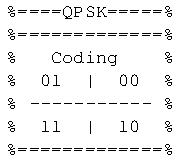
\includegraphics[width=0.3\linewidth]{qpsk_mapping.pdf}
  
}
\\ 
  \subfloat[\label{1b}]{%
    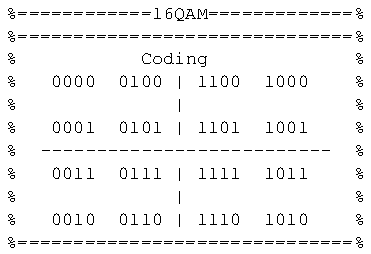
\includegraphics[width=0.6\linewidth]{qam16mapping.pdf}
}

  \caption{Symbol mapping for QPSK (a) and QAM-16 (b) modulated symbols}
  \label{fig:mapping} 
\end{figure}


The training sequence is added to both I and Q symbols in the block \textit{Add Barker}. The training sequence is an appropriate repetition of Barker sequences of length 7 and 13 for QPSK and QAM-16 modulation respectively. The total length of the training sequence is 26 symbols. 

In the last step before transmission, the symbols are upsampled by a factor $\sps$ and filtered with a pulse shaping filter. The filter is a Root Raised Cosine with a roll-off factor of 0.5. The same filter is applied as a matched filter in the first step at the receive side before the samples are downsampled again. 

The USRP is configured to transmit continuously with a symbol rate of $\symbolRateQPSK$ symbols per second and transmits I/Q zeros when no data is available. A \SI{100}{ms} USB buffer is used on both TX and RX side of the USRP to minimize the effects of USB-latency. The USRP interface is implemented using the NI-USRP DLL \cite{labviewDLL}.

Symbol synchronization is done by choosing the sample offset that maximizes the signal energy. 

Frame synchronization is done by computing the crosscorrelation between the two training sequences and the received symbols. After a frame is found, only the frame symbols are passed along to the next block.

\subsection{Frequency and Phase Synchronization}
The implemented frequency synchronization algorithm is based on the Mth-power algorithm\cite{viterbi}, which is further improved by using a Kalman filter. Frequency offset is estimated from the training sequence only. The Mth-power algorithm estimates the phase offset of MPSK modulated symbols by mapping all symbols to the same point in the complex plane. By tracking the angular difference between consecutive symbols, the frequency offset may be estimated. In our case, the QPSK symbols of the training sequence is raised to the 4th power, and the phase is estimated as indicated in figure \ref{fig:mth_pow}.
% !TEX root = main.tex
\begin{figure}[htbp]
\centering
\begin{tikzpicture}
% Grids
\coordinate (origo) at (0,0);
\coordinate (origo_w) at (5.1,0);

\draw[step=0.3cm,gray,very thin] (-1.51,-1.51) grid (1.5,1.5);
\draw[step=0.3cm,gray,very thin] (3.6,-1.51) grid (6.6, 1.5);

% Axis
\draw[thick, ->] (-1.5,0) -- (1.5, 0) node [anchor=north west]{\Re[$z$]};
\draw[thick, ->] (0,-1.5) -- (0,1.5) node [anchor=south west]{\Im[$z$]};
\draw[thick, ->] (3.6,0) -- (6.6, 0) node [anchor=north west]{\Re[$w$]};
\draw[thick, ->] (5.1,-1.5) -- (5.1,1.5) node [anchor=south west]{\Im[$w$]};

\draw[thick] (0.9, 0) ++(0, 2pt) -- ++(0,-4pt) node[font=\scriptsize, yshift=-0.1cm, xshift=-0.1cm]{1};
\draw[thick] (-0.9, 0) ++(0, 2pt) -- ++(0,-4pt) node[font=\scriptsize, yshift=-0.1cm, xshift=-0.1cm]{-1};
\draw[thick] (0, 0.9) ++(2pt, 0) -- ++(-4pt, 0) node[font=\scriptsize, yshift=-0.1cm, xshift=-0.1cm]{1};
\draw[thick] (0, -0.9) ++(2pt, 0) -- ++(-4pt, 0) node[font=\scriptsize, yshift=-0.1cm, xshift=-0.1cm]{-1};

\draw[thick] (6, 0) ++(0, 2pt) -- ++(0,-4pt) node[font=\scriptsize, yshift=-0.1cm, xshift=-0.1cm]{4};
\draw[thick] (4.2, 0) ++(0, 2pt) -- ++(0,-4pt) node[font=\scriptsize, yshift=-0.1cm, xshift=-0.1cm]{-4};
\draw[thick] (5.1, 0.9) ++(2pt, 0) -- ++(-4pt, 0) node[font=\scriptsize, yshift=-0.1cm, xshift=-0.1cm]{4};
\draw[thick] (5.1, -0.9) ++(2pt, 0) -- ++(-4pt, 0) node[font=\scriptsize, yshift=-0.1cm, xshift=-0.1cm]{-4};

% Plot
\draw[blue,fill=blue] (0.9,0.9) circle (2pt) coordinate[](sample);
\draw[blue,fill=blue] (-0.9,0.9) circle (2pt);
\draw[blue,fill=blue] (0.9,-0.9) circle (2pt);
\draw[blue,fill=blue] (-0.9,-0.9) circle (2pt);
\draw[red,fill=red] (0.73,1.043) circle (2pt) coordinate[](sample_err);

\draw[thin, blue] (0,0) -- (sample);
\draw[thin, red] (0,0) -- (sample_err);
\pic [draw, red, ->, angle eccentricity=1.5] {angle = sample--origo--sample_err};
\draw (0.3, 0.3) node[anchor=north west, text=red, yshift=0.2cm]{$\phi$};

\draw[blue,fill=blue] (3.83,0) circle (2pt) coordinate[](sample_w);
\draw[red,fill=red] (4.125,-0.818) circle (2pt) coordinate[](sample_err_w);
\draw[thin, blue] (origo_w) -- (sample_w);
\draw[thin, red] (origo_w) -- (sample_err_w);
\pic [draw, red, ->, angle eccentricity=1.5] {angle = sample_w--origo_w--sample_err_w};
\draw (origo_w) ++(-1.1,-0.35) node[anchor=north west, text=red, yshift=0.2cm]{$4\phi$};

% Other
\draw[thick, ->] (2, 1) .. controls (2.5,1.1) .. (3,1) node[above, anchor=south east, xshift=0.1cm]{$w=z^4$} ;

\end{tikzpicture}
\caption{Illustration the mapping $w=z^4$ which indicates how a phase error in QPSK modulated signal can be observed.}
\label{fig:mth_pow}
\end{figure}

For each received frame, the frequency offset is estimated by the mean of the angular difference between all consecutive symbols of the training sequence. The accuracy of the estimate is improved by the use of a Kalman filter.

After frequency correction, the phase offset is estimated as the mean of the angular deviation between the training sequence of the received symbols and the ideal Barker sequence.


